\chapter{态、可逆性与运动学}

经典力学并不仅仅是关于落体、行星轨道或带电粒子的一组方程。在选择任何具体方程之前，我们可以提出一个更一般的问题：一条运动定律必须是什么样子，才能算作经典定律？我们将从简单到可以把每一种可能的历史都画在黑板上的系统开始。一旦态、决定性、可逆性和守恒这些概念在那里变得清晰，我们就会回到在普通空间中运动的粒子。

\section{两类问题}

力学中有两类问题。一类要求给出支配某个特定系统的具体定律。在一个大质量天体的引力场中运动的行星遵循一种定律；在磁场中运动的带电粒子遵循另一种定律。这些是关于自然界具体定律的问题。

另一类问题涉及所有这些例子共有的框架。是否存在每一条允许的定律都必须满足的规则？哪些特征属于经典力学本身，而与所研究的力或物体无关？具体的例子将说明答案，但正是这第二类问题组织起了这门学科。

最有用的第一个例子是一枚抽象桌子上的抽象硬币。我们只保留硬币的一个属性：它可以显示正面或反面。因此它的构型空间是
\begin{equation}
  \mathcal C=\{H,T\}.
\end{equation}
\emph{构型}一词指的是系统可能处于的诸方式之一。初始条件就是对其中之一的选取。一枚单面硬币会更简单，但它只有一个构型，什么也不会发生。两个态就足以使动力学成为可能。

\section{硬币：态、定律与历史}

让时间以整数步前进，就好像世界被频闪仪照亮一样：
\begin{equation}
  t=\ldots,-2,-1,0,1,2,\ldots .
\end{equation}
运动定律是一条更新规则。它把时刻\(t\)的态指派给时刻\(t+1\)的态。最简单的规则什么也不做：
\begin{equation}
  H\longmapsto H,
  \qquad
  T\longmapsto T.
  \label{eq:coin-identity}
\end{equation}
从\(H\)出发，整个历史是\(H,H,H,\ldots\)；从\(T\)出发，它是\(T,T,T,\ldots\)。这条规则很无聊，但它完全具有预测性。

另一条可逆规则交换两个态：
\begin{equation}
  H\longmapsto T,
  \qquad
  T\longmapsto H.
  \label{eq:coin-flip}
\end{equation}
历史现在交替出现：
\begin{equation}
  H,T,H,T,\ldots,
  \qquad
  T,H,T,H,\ldots .
\end{equation}
箭头从更新前的态指向更新后的态。因此箭尾表示系统从哪里开始，箭头表示它到哪里去。

\begin{figure}[htbp]
  \centering
  \includegraphics[width=0.86\textwidth]{lecture_01_figure_02.png}
  \caption{硬币的两个构型以及讲台黑板上的有向翻转定律。干净的更新规则由式~\eqref{eq:coin-flip}给出。}
  \lectureframe{00:06:50}
  \label{fig:coin-board}
\end{figure}

我们可以用一个二值变量来编码两个面，
\begin{equation}
  \sigma=
  \begin{cases}
    +1,&H,\\
    -1,&T.
  \end{cases}
\end{equation}
字母\(\sigma\)在物理学中传统上用于二值量，尤其是在自旋的描述中，尽管这里不需要任何关于自旋的知识。在这种记号下，两条规则变成运动方程：
\begin{align}
  \sigma(t+1)&=\sigma(t),
  &&\text{identity law},\label{eq:sigma-identity}\\
  \sigma(t+1)&=-\sigma(t),
  &&\text{flip law}.\label{eq:sigma-flip}
\end{align}
这个变量并没有增添新的物理。它为构型提供了一个紧凑的标签，并把图变成方程。

\begin{figure}[htbp]
  \centering
  \includegraphics[width=0.86\textwidth]{lecture_01_figure_03.png}
  \caption{翻转定律写成
  \(\sigma(t+1)=-\sigma(t)\)。方框中的值\(\sigma=\pm1\)标记正面和反面。}
  \lectureframe{00:08:58}
  \label{fig:sigma-board}
\end{figure}

对任一条规则，初始态和定律都决定了此后每一时刻的态。这一陈述假定系统是\emph{封闭}的。如果有人伸手进来转动硬币，那么这只手就是一种外部影响，并未包含在我们的描述中。我们并没有推翻决定性；我们改变了系统。经典定律旨在支配一个封闭系统，其中包含所有与其演化相关的影响。

从二元集合到自身的数学函数共有四个。上面未写出的两个把两个输入都送到\(H\)，或者把两个输入都送到\(T\)。它们对未来是决定性的，但它们抹去了两种可能过去之间的区别。当下面施加可逆性时，式~\eqref{eq:coin-identity}和\eqref{eq:coin-flip}恰好就是两个允许的映射。

\section{骰子：轨道与守恒量}

把硬币换成骰子。就目前的目的而言，关于骰子唯一重要的事实是它有六个构型，
\begin{equation}
  \mathcal C=\{1,2,3,4,5,6\}.
\end{equation}
初始条件就是选取其中一个数。我们本可以再次让每个态保持不变，但对于不那么平凡的规则，有向图更有用。考虑
\begin{equation}
  1\longmapsto2\longmapsto3\longmapsto4
  \longmapsto5\longmapsto6\longmapsto1.
  \label{eq:six-cycle}
\end{equation}
例如从\(4\)出发，历史是

\[
  4,5,6,1,2,3,4,\ldots .
\]
这六个状态构成一个循环。\footnote{来源说明：在第一次阅读箭头时，有一句口头表述说\(6\)返回到\(6\)。紧接着的下一句、所画的循环以及列举的历史都给出预期的更新\(6\mapsto1\)。}

\begin{figure}[htbp]
  \centering
  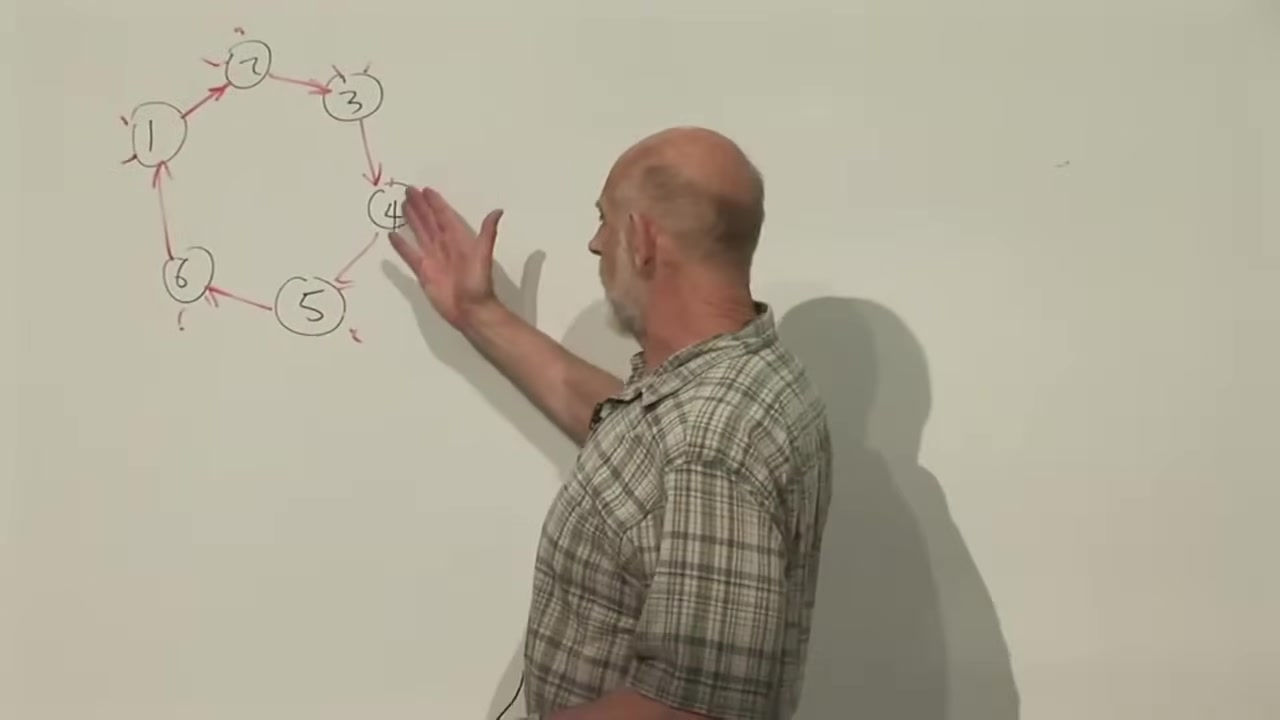
\includegraphics[width=0.86\textwidth]{lecture_01_figure_06.png}
  \caption{单一的六状态循环。每个频闪步，一个状态移动到下一个状态，并在六次更新后返回。}
  \lectureframe{00:12:40}
  \label{fig:six-cycle-board}
\end{figure}

一条规则可以看起来更复杂，但在结构上并无不同。例如，
\begin{equation}
  1\to2\to5\to3\to4\to6\to1
  \label{eq:relabeled-cycle}
\end{equation}
仍然是一个单一的六循环。如果按\(1,2,5,3,4,6\)的顺序把顶点放在页面上，它就变成与式~\eqref{eq:six-cycle}相同的图。诸如\(1\)和\(5\)这样的标签只是名称；循环结构并不依赖于它们。

一条真正不同的定律把六个状态分成两个循环，例如
\begin{equation}
  1\to2\to3\to1,
  \qquad
  4\to6\to5\to4.
  \label{eq:two-cycles}
\end{equation}
仍然只有一个骰子和一条定律，但从一个循环上开始的轨迹永远不能到达另一个循环。我们可以给这些循环附上一个数\(Q\)，
\begin{equation}
  Q=
  \begin{cases}
    0,&\text{on the cycle }\{1,2,3\},\\
    1,&\text{on the cycle }\{4,5,6\}.
  \end{cases}
\end{equation}
状态每一步都改变，而\(Q\)不改变。

\begin{definition}
守恒量是状态的一个函数，其值不被运动定律改变。
\end{definition}

同样的想法允许一个不动点、一个二循环和一个三循环。守恒标签说明系统占据哪条轨道；它不必标识该轨道内的状态。因此守恒与运动相容。被保持的不一定是完整的位形，而是可能位形之间的某种区分。

\begin{figure}[htbp]
  \centering
  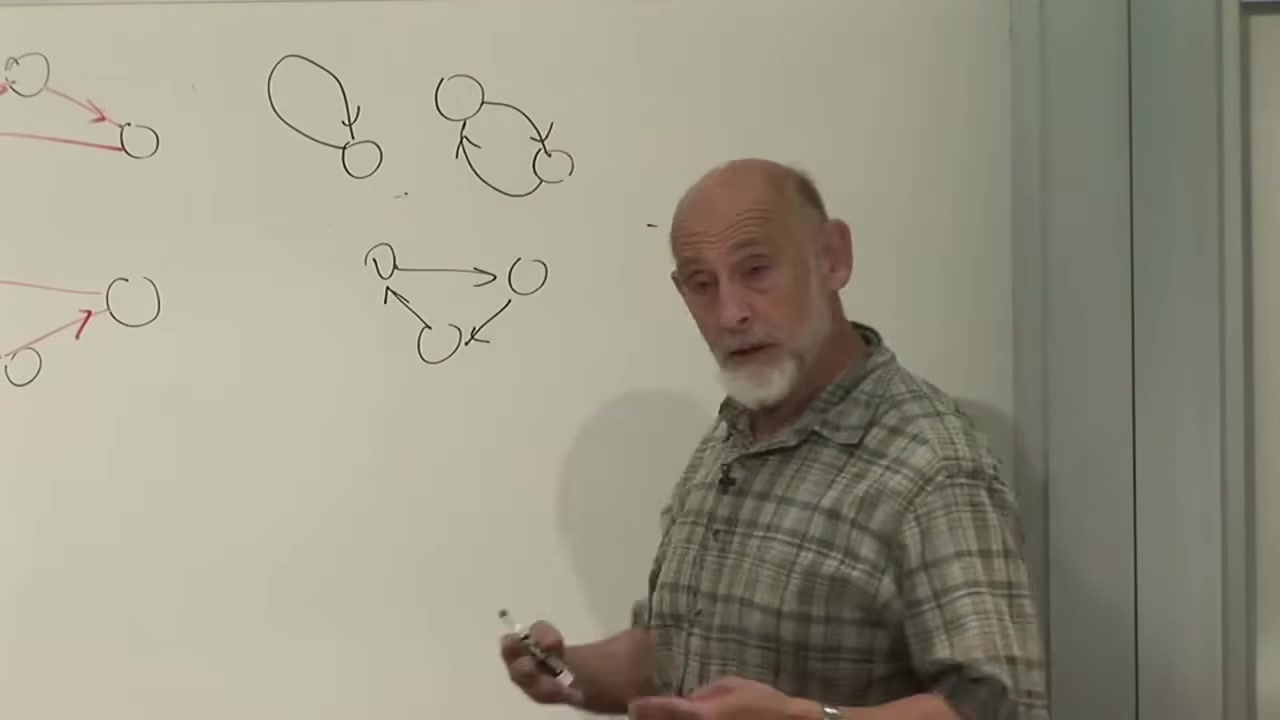
\includegraphics[width=0.86\textwidth]{lecture_01_figure_07.png}
  \caption{板上的几个不连通循环：一个不动点、一个二循环和一个三循环。即使状态沿其循环移动，循环标签也是守恒的。}
  \lectureframe{00:18:40}
  \label{fig:conserved-cycles-board}
\end{figure}

对于有限可逆系统，每条轨迹都是一个循环。单个循环没有这种初等意义上的非平凡守恒标签，因为轨迹最终会访问每一个状态。多个循环允许这样的标签，因为演化绝不会把一个状态从一个连通分量带到另一个连通分量。

\section{状态中必须包含什么？}

硬币例子使用的是一步规则：下一面只依赖于当前面。听众提出的一个问题检验这一限制是否本质。

\begin{classroomqa}
\audiencequestion{能否构造一个正面和反面的序列，使得下一个结果依赖于不止当前可见的面，也许依赖于一个或几个更早的结果？\lecturetimestamp{00:19:27--00:21:23}}

\lecturerresponse{可以。在这种情况下，仅\(H\)或仅\(T\)不是完整状态。如果需要前一个面，就把状态空间扩大为
\(
  \{HH,HT,TH,TT\}.
\)
每个有序对记录当前面和前一个面。于是演化又可以写为这个四状态空间上的一步规则。如果还需要更多历史，也把那些信息包括进去。}
\end{classroomqa}

这个回答给出了状态的操作性含义。

\begin{definition}
系统在某一时刻的状态由所有所需信息组成，这些信息与运动定律一起足以预测其未来。
\end{definition}

因此，状态不仅仅是一张照片。它是使演化确定的任何完整数据集。以后，当我们描述一个牛顿粒子时，仅其位置将不够；速度也将属于初始数据。带记忆的硬币是同一原理的最简单版本。

\section{无限状态空间}

无限多个状态并不要求无限多个物体。取一个被约束在无限直线上的整数格点的粒子。它的状态是一个整数
\[
  n\in\mathbb Z.
\]
一条定律使它每一步向右移动一个格点：
\begin{equation}
  n(t+1)=n(t)+1.
  \label{eq:lattice-one}
\end{equation}
这条轨道永不闭合，但如果同时沿未来和过去追踪，它会经过每一个整数。在这种扩展的意义上，它扮演一个无尽循环的角色。

另一条定律每次移动两个格点：
\begin{equation}
  n(t+1)=n(t)+2.
  \label{eq:lattice-two}
\end{equation}
现在偶格点只在偶格点之间演化，奇格点只在奇格点之间演化。宇称是守恒的：
\begin{equation}
  \begin{aligned}
    Q_{\rm parity}(n)&=n\bmod 2,\\
    Q_{\rm parity}(n(t+1))&=Q_{\rm parity}(n(t)).
  \end{aligned}
\end{equation}
从有限位形空间到无限位形空间的过渡允许永不重复的历史，但它不改变状态、轨道或守恒的含义。

\section{确定性尚不是可逆性}

我们现在画出一条规则，它能唯一地预测未来，却不满足第二条经典要求。给一枚三面硬币赋予正面、反面和边缘三个状态，并定义
\begin{equation}
  H\to T,
  \qquad
  T\to E,
  \qquad
  E\to T.
  \label{eq:nonreversible-map}
\end{equation}
从\(H\)出发，历史是
\[
  H,T,E,T,E,\ldots;
\]
从\(T\)或\(E\)出发，随后的交替同样明确无误。每个状态恰好有一条出射箭头，因此该规则对未来是确定性的。

当我们试图重构过去时，困难就出现了。如果当前状态是\(T\)，那么前一状态可能是\(H\)或\(E\)。两条历史合并了。把每条箭头都反向，缺陷立刻显现：从\(T\)出发，反向图提供两种可能的移动。反向规则不是确定性的。

\begin{figure}[htbp]
  \centering
  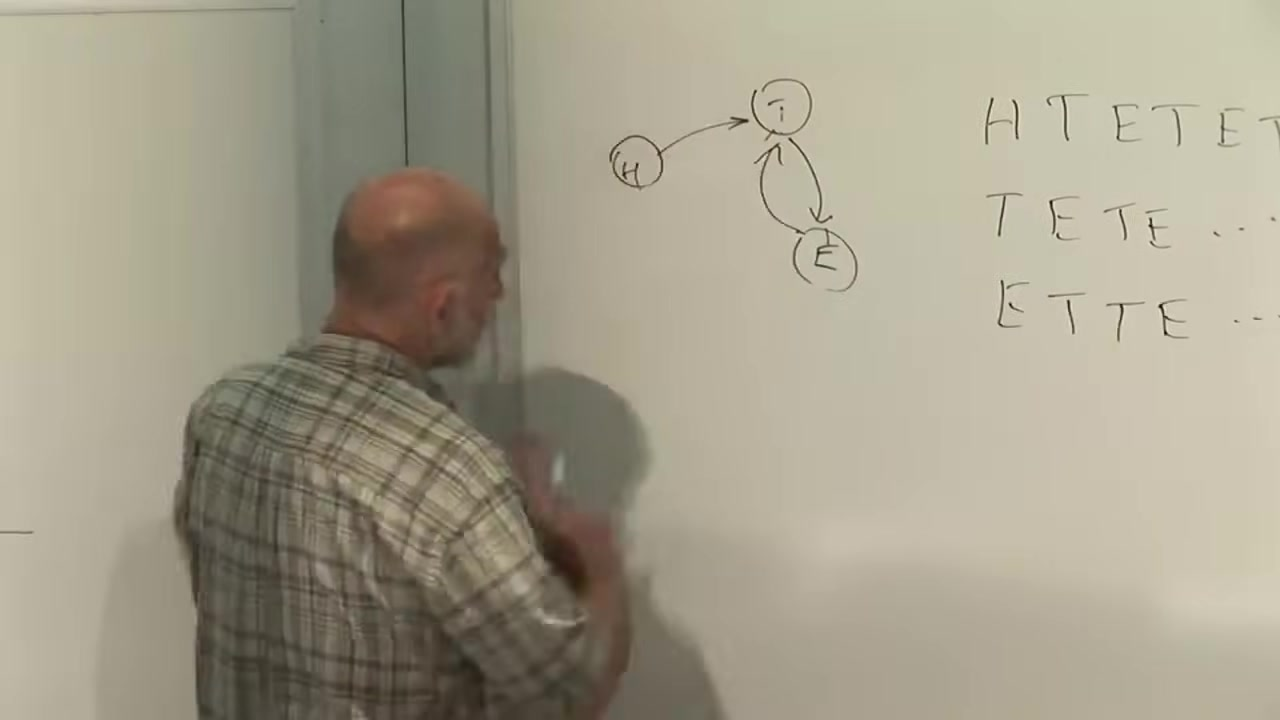
\includegraphics[width=0.86\textwidth]{lecture_01_figure_08.png}
  \caption{不可逆的\(H,T,E\)定律与代表性历史。
  \(H\)和\(E\)都汇入\(T\)，因此现在并不决定唯一的过去。}
  \lectureframe{00:28:50}
  \label{fig:nonreversible-board}
\end{figure}

\begin{definition}
当现在状态既决定唯一的下一状态又决定唯一的前一状态时，离散定律是可逆的。在状态图中，每个状态必须恰好有一条出射箭头和恰好一条入射箭头。
\end{definition}

对于有限状态空间，可逆更新是状态的一个置换。它从不创造或消灭状态之间的区别；它只是重新排列它们。这就是为什么它的图分解为循环。式~\eqref{eq:nonreversible-map}中的映射是一个函数，但不是一一函数，因此没有逆。

\begin{classroomqa}
\audiencequestion{如果这种规则所表示的状态是粒子的概率，它能否被允许？\lecturetimestamp{00:29:46--00:31:17}}

\lecturerresponse{那将是另一种框架。这里所表述的基本经典力学使用确定性定律，而不是概率性更新规则。人们当然可以发明并研究这样的规则，但在这个意义上它不是经典力学定律。量子力学不以同样的方式确定，然而它也有可逆演化的类似物；那需要以后的讨论。经典统计力学也使用概率，但它从底层的力学定律出发，并表示对它们初始数据的不完全知识。}
\end{classroomqa}

这一区分很重要。因为我们不知道确切的经典状态而使用的概率分布，并不是非确定性的运动定律。它描述的是我们对一个系统的信息，而该系统的微观演化仍被视为确定且可逆的。

\section{精确定律与不完善知识}

预测需要两个要素：
\begin{enumerate}
  \item 运动定律；
  \item 初始状态。
\end{enumerate}
当初始条件只能近似知道时，精确定律不会产生精确预报。对于硬币，很容易想象看着桌面并完全得知其面。真实的力学变量是连续的。位置和速度可以取任意实数值，而没有任何测量能提供无穷多位小数。

假设真实的初始状态位于一个小的可能状态区域内。在某些动力学下，该区域长时间保持很小；在另一些动力学下，邻近的初始状态迅速分离。在混沌系统中，小的初始不确定性最终会增长为大的差异。大气是一个熟悉的例子。更好的测量可以延长有用的预报，但对于任何固定的测量精度，都存在一个足够遥远的时间，使预报变得不可靠。

这种实际限制并不会给方程引入歧义。如果初始条件被精确知道，经典可逆定律将同时决定未来和过去。在有限精度下，定量问题反而是：为了对指定长度的时间作出预测，初始状态必须被知道得多么精确？

图形检验现在有一个简洁的结论。在每个状态都由一条入射箭头和一条出射箭头表示的定律是确定且可逆的。关于粒子的相应陈述将不那么初等，但它们表达同样的经典结构。

\section{从抽象状态到空间中的点}

接下来我们从硬币和骰子转向质点。质点可以在1维、3维、5维或任意其他维数中运动，但普通空间提供了最直接的例子。为了定量地描述一个点，需要选择：
\begin{itemize}
  \item 一个原点；
  \item 三条相互垂直的轴；
  \item 这些轴的一个取向；
  \item 一个长度单位。
\end{itemize}
原点是约定性的。它可以放在帕洛阿尔托或任何其他地方，物理结论不应依赖于这一选择。这些轴可以标记为\(x,y,z\)，或\(x_1,x_2,x_3\)。在\(x\)方向和\(y\)方向确定之后，\(z\)轴可以指向两个垂直方向中的任意一个。我们采用右手约定：右手拇指沿\(x\)，食指沿\(y\)，则中指指向\(z\)。

沿各轴的等距标记需要一个单位，例如米、英尺、英寸或光年。一旦这些约定固定下来，每个点就由三个数标记，
\begin{equation}
  (x,y,z).
\end{equation}
人们可以从原点出发，沿三条轴通过位移到达该点。一个由许多质点组成的系统需要为每个质点提供这样一组三元数。

\begin{figure}[htbp]
  \centering
  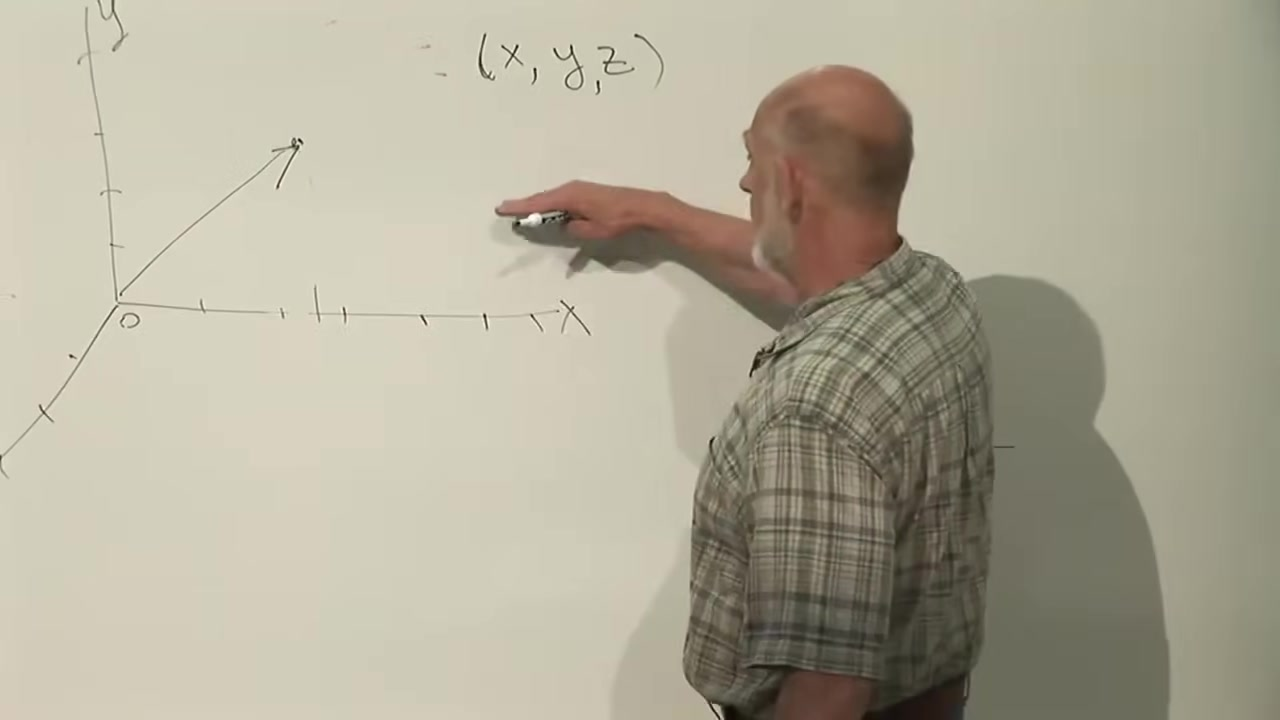
\includegraphics[width=0.86\textwidth]{lecture_01_figure_09.png}
  \caption{笛卡尔坐标轴与一个点的三个坐标。该图固定了一种坐标约定；点本身并不依赖于我们选择把原点或轴放在哪里。}
  \lectureframe{00:43:00}
  \label{fig:coordinates-board}
\end{figure}

\section{矢量及其分量}

矢量是具有大小和方向的客体。从原点到某一点的位移是一个矢量，但矢量也描述速度、加速度、电场以及许多其他量。我们将用粗体书写矢量，例如\(\mathbf v\)，其大小写作\(\lvert\mathbf v\rvert\)。大小是非负的，并且仅对零矢量才为零。

从几何上看，矢量是一支自由箭头。平移这支箭头而不改变其长度或方向，不会改变该矢量。在特定应用中，矢量可以附着于一个点，例如当我们指定给定位置处的电场时，但附着是额外的信息，并不是抽象矢量本身的一部分。

相对于笛卡尔坐标轴，一个矢量具有分量
\begin{equation}
  \mathbf v=(v_x,v_y,v_z).
\end{equation}
这些分量是普通的带符号数，通过在各轴上的投影得到。它们同时编码了大小和方向。三维勾股定理给出
\begin{equation}
  \lvert\mathbf v\rvert^2
  =v_x^2+v_y^2+v_z^2,
  \qquad
  \lvert\mathbf v\rvert
  =\sqrt{v_x^2+v_y^2+v_z^2}.
  \label{eq:vector-magnitude}
\end{equation}
各分量的比值决定方向。一个负分量意味着该矢量部分地指向该轴的负方向。

\subsection{标量乘法与加法}

乘以一个实数会改变矢量的长度，并且如果该数为负，还会反转其方向。对于\(c>0\)，\(c\mathbf A\)指向\(\mathbf A\)的方向，且大小为
\(c\lvert\mathbf A\rvert\)。特别地，\(-\mathbf A\)与\(\mathbf A\)长度相同，但指向相反。

矢量加法有三种等价的图像。第一，把\(\mathbf B\)的尾端放在\(\mathbf A\)的首端；从\(\mathbf A\)的尾端到\(\mathbf B\)的首端的箭头就是\(\mathbf A+\mathbf B\)。第二，把两者的尾端放在一起并补成一个平行四边形；其对角线就是和。这种形式使交换律显而易见：
\begin{equation}
  \mathbf A+\mathbf B=\mathbf B+\mathbf A.
\end{equation}
第三，把对应分量相加：
\begin{equation}
  C_i=A_i+B_i,
  \qquad i=x,y,z,
  \label{eq:component-addition}
\end{equation}
其中\(\mathbf C=\mathbf A+\mathbf B\)。这些规则也定义了任意线性组合，例如\(a\mathbf A+b\mathbf B\)。

\begin{figure}[htbp]
  \centering
  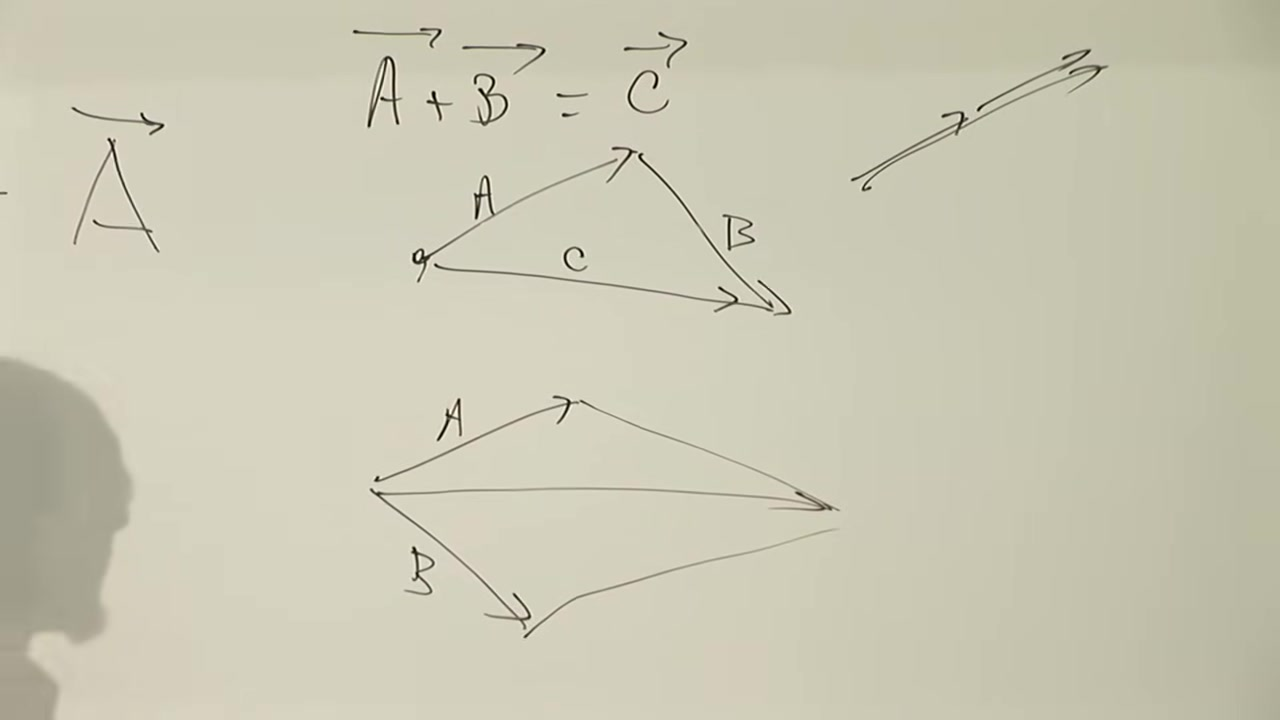
\includegraphics[width=0.86\textwidth]{lecture_01_figure_10.png}
  \caption{矢量加法的三角形构造与平行四边形构造。两者给出同一个矢量\(\mathbf A+\mathbf B\)。}
  \lectureframe{00:53:00}
  \label{fig:vector-addition-board}
\end{figure}

并不存在将一个矢量除以另一个矢量的一般运算。然而，有两种标准的矢量乘积。叉积将留到以后的讲座。这里我们需要点积。

\subsection{点积}

把\(\mathbf A\)投影到由\(\mathbf B\)定义的轴上。如果两矢量之间的夹角为\(\theta\)，则\(\mathbf A\)沿\(\mathbf B\)的带符号分量为\(\lvert\mathbf A\rvert\cos\theta\)。将此投影乘以\(\lvert\mathbf B\rvert\)，定义为
\begin{equation}
  \mathbf A\cdot\mathbf B
  =\lvert\mathbf A\rvert\,\lvert\mathbf B\rvert\cos\theta.
  \label{eq:dot-geometric}
\end{equation}
结果是一个标量，而不是另一个矢量。式~\eqref{eq:dot-geometric}对\(\mathbf A\)和\(\mathbf B\)是对称的，所以\(\mathbf A\cdot\mathbf B=\mathbf B\cdot\mathbf A\)。

\begin{figure}[htbp]
  \centering
  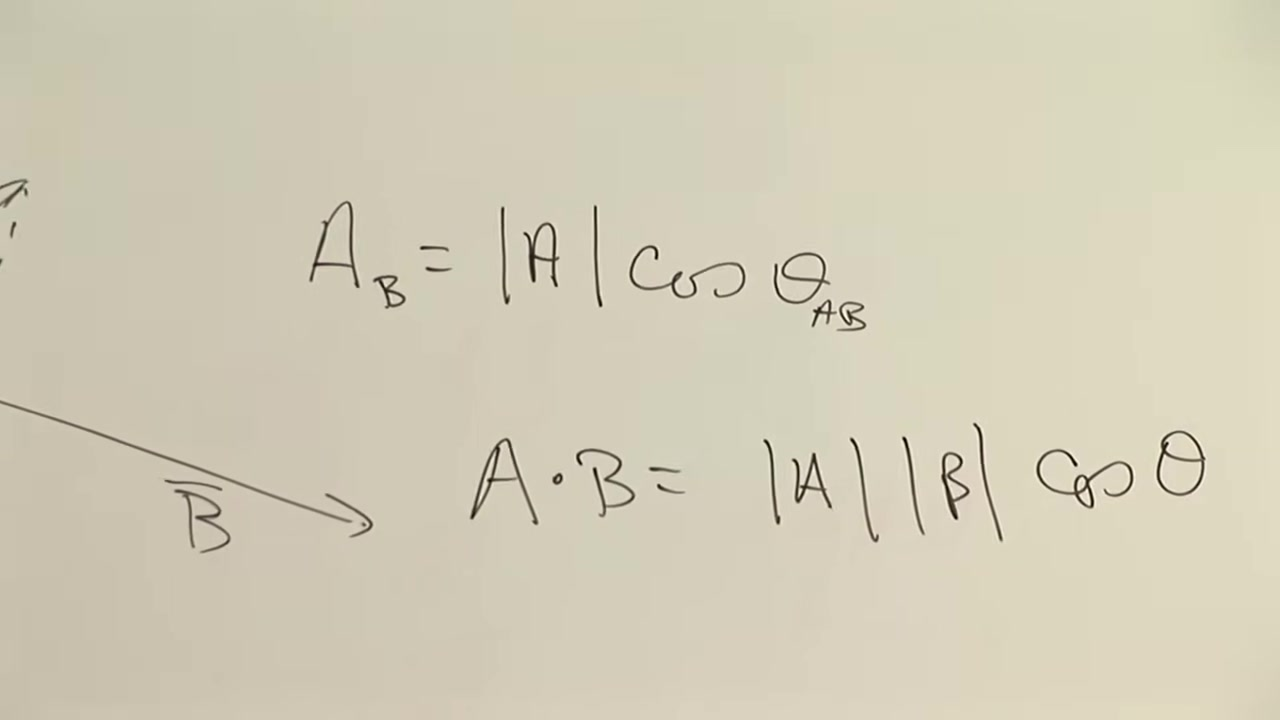
\includegraphics[width=0.86\textwidth]{lecture_01_figure_11.png}
  \caption{黑板上通过投影构造点积的过程。排版形式为
  \(\mathbf A\cdot\mathbf B=AB\cos\theta\)。}
  \lectureframe{00:58:30}
  \label{fig:dot-product-board}
\end{figure}

符号携带几何信息。对于锐角，点积为正；对于钝角，点积为负；对于垂直矢量，点积为零。因此，对于非零矢量，
\begin{equation}
  \mathbf A\perp\mathbf B
  \quad\Longleftrightarrow\quad
  \mathbf A\cdot\mathbf B=0
\end{equation}

写成分量形式，
\begin{equation}
  \mathbf A\cdot\mathbf B
  =A_xB_x+A_yB_y+A_zB_z.
  \label{eq:dot-components}
\end{equation}
这个公式使计算变得直接。特别地，
\begin{equation}
  \mathbf A\cdot\mathbf A
  =A_x^2+A_y^2+A_z^2
  =\lvert\mathbf A\rvert^2.
  \label{eq:self-dot}
\end{equation}
给定两个向量的分量，式~\eqref{eq:dot-geometric}和
\eqref{eq:dot-components}就确定了它们之间的夹角：
\begin{equation}
  \cos\theta
  =\frac{\mathbf A\cdot\mathbf B}
  {\lvert\mathbf A\rvert\,\lvert\mathbf B\rvert}.
\end{equation}

余弦定理可由同样的代数运算得到。设\(\mathbf A\)和
\(\mathbf B\)从同一个顶点出发，指向三角形的另外两个顶点。第三条边是
\(\mathbf C=\mathbf A-\mathbf B\)，而不是\(\mathbf A+\mathbf B\)。因此
\begin{align}
  C^2
  &=(\mathbf A-\mathbf B)\cdot(\mathbf A-\mathbf B)\notag\\
  &=A^2+B^2-2\mathbf A\cdot\mathbf B\notag\\
  &=A^2+B^2-2AB\cos\theta.
  \label{eq:law-of-cosines}
\end{align}

\begin{figure}[htbp]
  \centering
  \includegraphics[width=0.86\textwidth]{lecture_01_figure_04.png}
  \caption{用于余弦定理的三角形。板书更正
  将闭合边确定为
  \(\mathbf C=\mathbf A-\mathbf B\)，由此得到
  式~\eqref{eq:law-of-cosines}。}
  \lectureframe{01:04:29}
  \label{fig:law-cosines-board}
\end{figure}

\section{位置、速度与加速度}

选定一个原点，设\(\mathbf r\)为从原点到质点的位置矢量。其分量就是笛卡尔坐标：
\begin{equation}
  \mathbf r=(x,y,z),
  \qquad
  \lvert\mathbf r\rvert=\sqrt{x^2+y^2+z^2}.
\end{equation}
改变原点会改变\(\mathbf r\)，这个问题我们留待以后讨论。一旦
原点固定，运动就由依赖于时间的位置来描述，
\begin{equation}
  \mathbf r(t)=\bigl(x(t),y(t),z(t)\bigr).
\end{equation}
因此轨迹由三个关于时间的函数编码。

速度是位置对时间的导数：
\begin{equation}
  \mathbf v(t)=\frac{d\mathbf r}{dt}
  =\dot{\mathbf r}(t),
  \qquad
  v_i=\frac{dx_i}{dt}=\dot x_i.
  \label{eq:velocity}
\end{equation}
点号始终表示对时间的导数。大小
\(\lvert\mathbf v\rvert\)就是速率。位置和速度一般是相互独立的
方向：位于某一位置的质点可以沿问题所允许的任意
方向运动。

加速度是速度的变化率，因而也是位置对时间的二阶
导数：
\begin{equation}
  \mathbf a(t)=\frac{d\mathbf v}{dt}
  =\dot{\mathbf v}(t)
  =\frac{d^2\mathbf r}{dt^2}
  =\ddot{\mathbf r}(t),
  \qquad
  a_i=\ddot x_i.
  \label{eq:acceleration}
\end{equation}
加速度也是矢量。如果沿正
\(x\)方向运动的质点加速，则\(a_x>0\)。如果它减速，则\(a_x<0\)。通常
所说的减速，不过就是与当前速度方向相反的加速度。更一般地说，即使
速度的大小保持不变，它也可以因方向的改变而改变。

\begin{figure}[htbp]
  \centering
  \includegraphics[width=0.86\textwidth]{lecture_01_figure_05.png}
  \caption{速度分量写成位置分量的时间导数。
  用紧凑的矢量记号表示，
  \(\mathbf v=d\mathbf r/dt\)。}
  \lectureframe{01:14:24}
  \label{fig:velocity-board}
\end{figure}

\subsection{直线上的匀加速运动}

对于一维运动，写
\begin{equation}
  x(t)=a+bt+ct^2.
  \label{eq:quadratic-motion}
\end{equation}
在\(t=0\)时，质点位于\(x=a\)。求一次导再求一次导
得到
\begin{align}
  v(t)=\dot x(t)&=b+2ct,\label{eq:line-velocity}\\
  a(t)=\ddot x(t)&=2c.\label{eq:line-acceleration}
\end{align}
因此\(b\)是初速度，\(2c\)是恒定加速度。如果
\(c>0\)，速度线性增加；如果\(c<0\)，它线性减小。
这个二次位置规律就是恒定加速度下运动所取的形式，例如地球
表面附近落体的理想化运动。

\section{匀速圆周运动}

作为最后一个例子，设质点沿\(x\)-\(y\)平面内的
单位圆运动。它在\(t=0\)时从正\(x\)轴出发，其角
坐标均匀增加：
\begin{equation}
  \theta(t)=\omega t.
\end{equation}
常数\(\omega\)是角频率。转一整圈对应于角度增加
\(2\pi\)，所以周期为
\begin{equation}
  T=\frac{2\pi}{\omega}.
  \label{eq:circular-period}
\end{equation}
可以允许角度增大到超过\(2\pi\)；位置会重复，
尽管连续记录的角度并不复位。

在单位圆上，
\begin{equation}
  \mathbf r(t)
  =\bigl(\cos\omega t,\,\sin\omega t\bigr).
  \label{eq:circular-position}
\end{equation}
求导得到
\begin{equation}
  \mathbf v(t)
  =\omega\bigl(-\sin\omega t,\,\cos\omega t\bigr).
  \label{eq:circular-velocity}
\end{equation}
速度与圆相切。我们可以不依赖图形来证明它与
半径垂直：
\begin{align}
  \mathbf r\cdot\mathbf v
  &=\cos\omega t\,(-\omega\sin\omega t)
    +\sin\omega t\,(\omega\cos\omega t)\notag\\
  &=0.
  \label{eq:r-dot-v}
\end{align}

\begin{figure}[htbp]
  \centering
  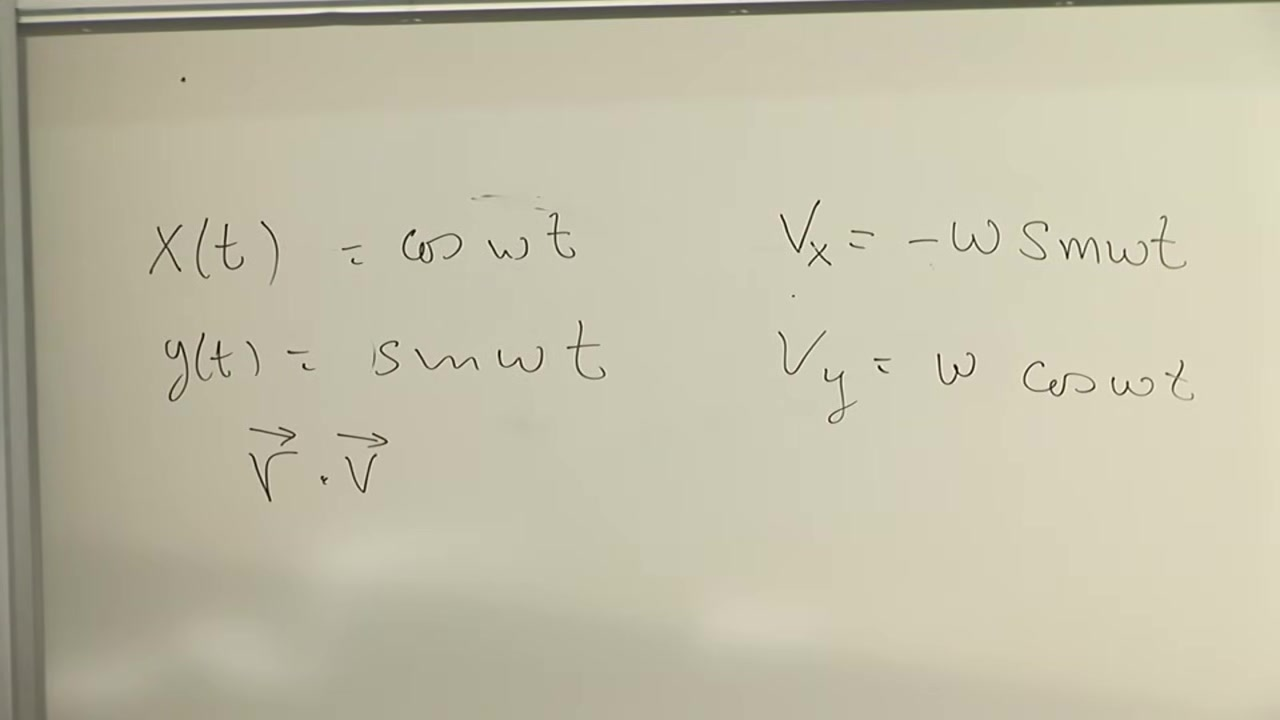
\includegraphics[width=0.86\textwidth]{lecture_01_figure_12.png}
  \caption{单位圆上运动的位置和速度分量。
  \(\mathbf r\cdot\mathbf v\)中的相消验证了速度
  与圆相切。}
  \lectureframe{01:24:30}
  \label{fig:circular-velocity-board}
\end{figure}

再求一次导，
\begin{equation}
  \mathbf a(t)
  =-\omega^2
  \bigl(\cos\omega t,\,\sin\omega t\bigr)
  =-\omega^2\mathbf r(t).
  \label{eq:centripetal-acceleration}
\end{equation}
加速度与半径平行，但指向相反的
方向，即指向圆心。这就是向心加速度。\footnote{术语
说明：讲到这里时讲座中出现了``离心''一词，但
方程和随附的描述所确定的是标准的向心
加速度，指向圆心。}

\begin{figure}[H]
  \centering
  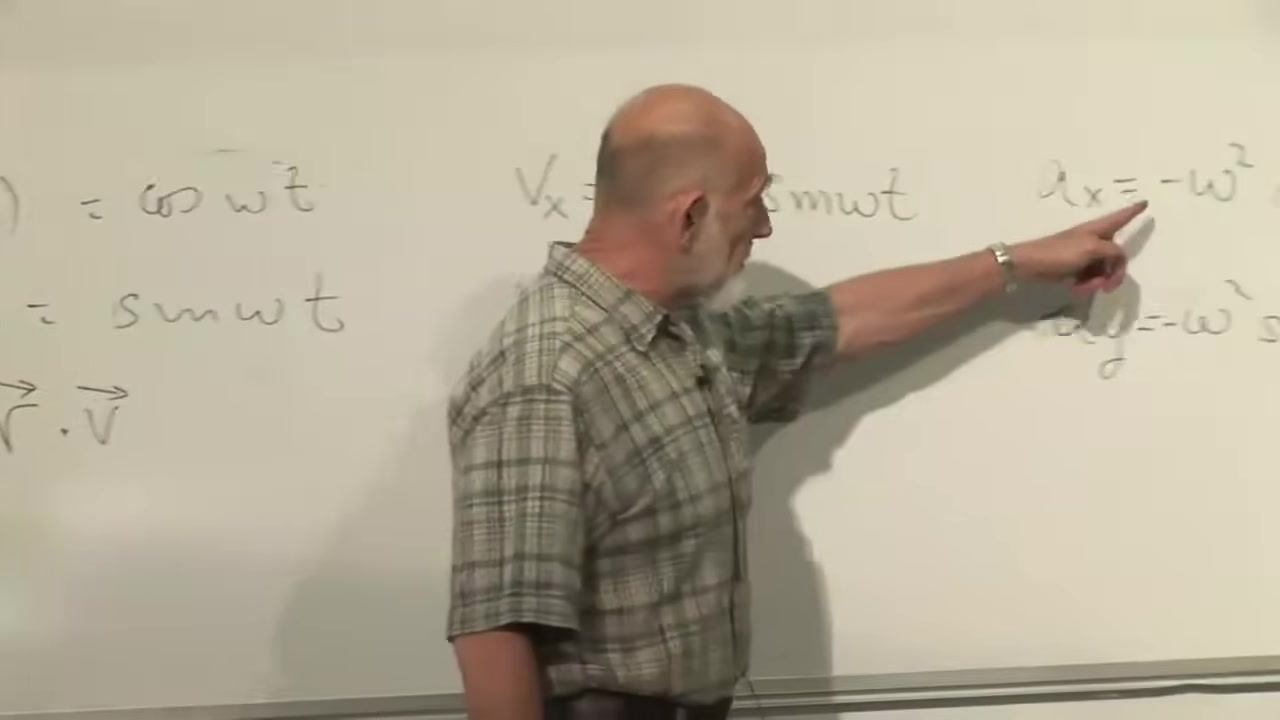
\includegraphics[width=0.86\textwidth]{lecture_01_figure_13.png}
  \caption{圆周运动加速度的分量计算。每个
  分量都是\(-\omega^2\)乘以相应的位置分量，所以
  \(\mathbf a=-\omega^2\mathbf r\)。}
  \lectureframe{01:26:30}
  \label{fig:circular-acceleration-board}
\end{figure}

因为半径为1，
\begin{equation}
  \lvert\mathbf r\rvert=1,
  \qquad
  \lvert\mathbf v\rvert=\omega,
  \qquad
  \lvert\mathbf a\rvert=\omega^2.
\end{equation}
增大\(\omega\)会使速率线性增大，而使所需的向内
加速度按二次方增大。对于半径为\(R\)的圆，同样的计算
会给出\(v=\omega R\)和
\(\lvert\mathbf a\rvert=\omega^2R=v^2/R\)；讲座取\(R=1\)是为了让
第一次计算保持简洁。

我们现在已经具备了粒子力学所需的基本语言：状态与初始数据、可逆演化、坐标、矢量，以及定义速度和加速度的导数。接下来的任务是确切判定哪些初始数据能够确定一个粒子，并找出把这些数据从一个时刻带到下一个时刻的定律。